\documentclass[conference]{IEEEtran}
%\documentclass[sigconf]{acmart}
\makeatletter
\def\ps@headings{%
\def\@oddhead{\mbox{}\scriptsize\rightmark \hfil \thepage}%
\def\@evenhead{\scriptsize\thepage \hfil \leftmark\mbox{}}%
\def\@oddfoot{}%
\def\@evenfoot{}}
\makeatother
\pagestyle{empty}
\usepackage{url}
\usepackage{graphicx,subfigure}
\usepackage{epstopdf}
\usepackage{amsmath}
\usepackage{algorithm}
\usepackage{algpseudocode}
\usepackage{amsmath}
\usepackage{amssymb}
\usepackage{amsthm}
\usepackage{epsfig}
\usepackage{tikz}
\usetikzlibrary{shapes, arrows, positioning}
\newtheorem{theorem}{Theorem}
\renewcommand{\algorithmicrequire}{\textbf{Input:}} % Use Input in the format of Algorithm
\renewcommand{\algorithmicensure}{\textbf{Output:}} % Use Output in the format of Algorithm
\usepackage{amsfonts}
%\newtheorem{theorem}{Theorem}[section]
\newtheorem{mydef}{Definition}[section]
%\newtheorem{lemma}{Lemma}[section]
\usepackage{multirow}
\usepackage{color}
\usepackage{array}
\usepackage{listings}
\usepackage{hyperref}
\usepackage[underline=true]{pgf-umlsd}
\newcommand{\tabincell}[2]
{\begin{tabular}
		{@{}#1@{}}#2\end{tabular}}
\usepackage{setspace}
\renewcommand{\labelitemi}{$\vcenter{\hbox{\tiny$\bullet$}}$}

\hyphenation{op-tical net-works semi-conduc-tor}

\begin{document}

\title{Time Series Price Prediction}

\author{\IEEEauthorblockN{1\textsuperscript{st} John Rizzo}
\IEEEauthorblockA{\textit{Dept. of Computer Science (of Aff.)} \\
\textit{Stevens Institute of Technology (of Aff.)}\\
Hoboken, USA \\
jrizzo2@stevens.edu}
\and
\IEEEauthorblockN{2\textsuperscript{nd} Matthew Kawaja}
\IEEEauthorblockA{\textit{Dept. of Computer Science (of Aff.)} \\
\textit{Stevens Institute of Technology (of Aff.)}\\
Hoboken, USA \\
mkawaja@stevens.edu}
\and
\IEEEauthorblockN{3\textsuperscript{rd} Leor Yomtobian}
\IEEEauthorblockA{\textit{Dept. of Computer Science (of Aff.)} \\
\textit{Stevens Institute of Technology (of Aff.)}\\
Hoboken, USA \\
lyomtobi@stevens.edu}
}

\maketitle

\begin{abstract}
The objective of our research is to develop a SOTA model using deep learning techniques that matches or exceeds existing methods such as Ordinary Least Squares (OLS) and Patch Time Series Transformer (PatchTST) using only the daily OHCLV (Open, High, Low, Close, Volume) features supplemented with additional custom features that can be generated from this data.  During our research we have implemented OLS, PatchTST and a custom LSTM deep learning architecture.  The custom LSTM deep learning model did in fact exceed the performance of both OLS and PatchTST while at the same time being generalizable to additional assets.
\end{abstract}

\section{Introduction}

Financial market forecasting is notoriously difficult due to chaotic, noisy, and nonlinear data. Historically, statistical models such as ARIMA and GARCH were used, often assuming linear, stationary data. More recently, machine learning and deep learning, including Random Forests, SVMs, and LSTMs, have emerged, showing promise in capturing complex, non-linear dependencies. While powerful, these newer methods typically require more data and computation, and can be less transparent than traditional models.

The objective of this research is to develop deep learning models that are capable of outperforming techniques such as OLS and PatchTST, using the OHLCV data. This constraint focuses on the price features that are available and avoids relying on external indicators. Our methodology includes three different models. The first is an OLS regressing model, next is a PatchTST model, and the third is a custom LSTM deep learning model that focuses on financial data. PatchTST is effective at capturing temporal patterns across long sequences. However, it is very limited when it is applied to financial data that have many shifts and structural breaks in the data. Our LSTM model adds multiple hidden layers to better adapt to temporal variability and nonlinear dependencies in asset prices. 

We evaluated these models using historical price data. Metrics such as Mean Squared Error (MSE), Mean Absolute Error (MAE), and directional accuracy were used to assess the predictive performance of the model. Our custom LSTM model consistently outperforms both OLS and PatchTST across multiple assets, showing superior generalization and stability in volatile market conditions. This model shows strong potential, making it a viable candidate for real-world forecasting applications. 

\section{Related Work}

Recent advances in deep learning have further revolutionized the prediction of the stock market. Architectures such as Recurrent Neural Networks (RNNs), particularly Long Short-Term Memory (LSTM) networks, are well-suited for time-series data due to their ability to capture long-term dependencies. Convolutional Neural Networks (CNNs) have also found applications in analyzing stock chart patterns. Transformer models are even being explored for sentiment analysis from financial news. These deep learning approaches often improve accuracy, but come with challenges such as data quality, overfitting, and high computational costs.

The pursuit of more interpretable yet accurate models has led to hybrid models, which combine the strengths of different techniques. For instance, some approaches integrate traditional statistical methods with machine learning or deep learning algorithms, or use CNNs with LSTMs to capture both spatial and temporal features. The goal is to balance predictive capability with transparency.

Furthermore, Reinforcement Learning (RL) is emerging as a promising paradigm for financial trading and portfolio management. RL agents learn to make sequential decisions by interacting with a dynamic environment, adapting to changing market conditions and optimizing long-term investment strategies.

\section{Our Solution}

\subsection{Description of Dataset}

For the PatchTST and LSTM models the paperswithbacktest/Bonds-Daily-Price and paperswithbacktest/Stocks-Daily-Price datasets were used. The Stocks-Daily-Price dataset has over 24.3 million rows each containing the symbol, date, open, high, low, close, and adj\_close. The Bonds-Daily-Price dataset has the same fields as the Stocks-Daily-Price with the addition of a volume column and has 1.36M rows.  Both the Bonds-Daily-Price and Stocks-Daily-Price datasets were filtered to only cover the time from January 1st 2002 to June 28th 2025 and Apple (AAPL) for equities and the 10 year US Treasury Bond.  The OLS model used historical "Close" prices from Yahoo Finance for Apple (AAPL), Microsoft (MSFT), Alphabet (GOOG), and the iShares 20+ Year Treasury Bond ETF (TLT), covering October 1, 2024, to March 26, 2025. 
\begin{figure}
    \centering
    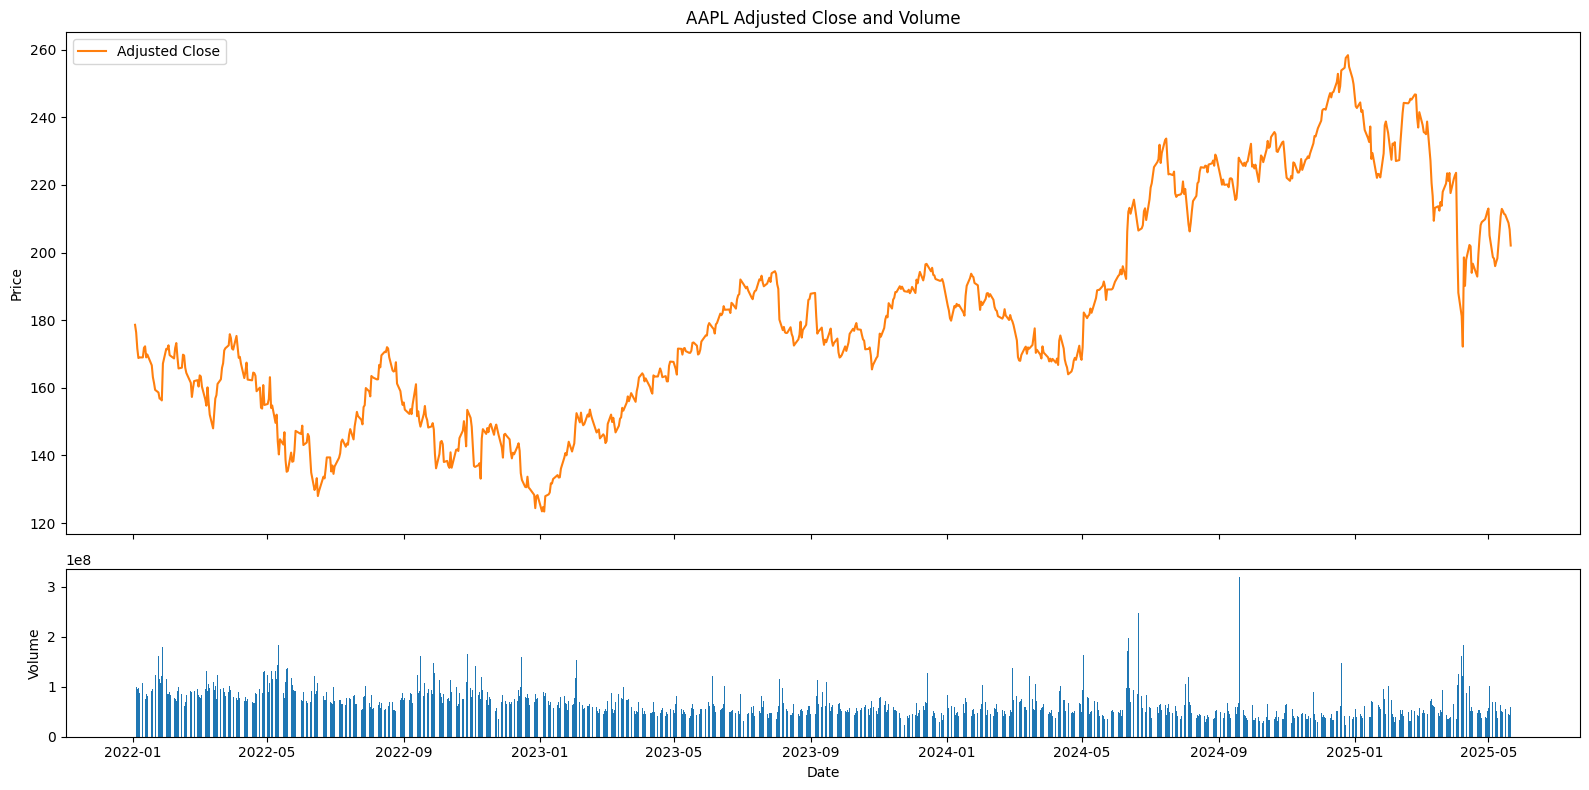
\includegraphics[width=1\linewidth]{aapl_adj_close_vs_volume.png}
    \label{fig:enter-label}
\end{figure}

Data preprocessing is crucial as these algorithms do not respond well to data with missing values and can be sensitive to extreme or unseen circumstances. We handle missing values (weekends/holidays) using a two-step forward (ffill) then backward (bfill) fill, ensuring a continuous time series. Feature engineering transforms raw prices into actionable attributes: lagged values (up to 5 days) capture history, rolling means (5-day window) indicate trends, and daily returns normalize price movements. Our target Key Performance Indicators (KPIs) are the next day's average tech stock return and bond price change, obtained by shifting these metrics backward by one day (.shift(-1)) to ensure prediction from past data. Finally, any remaining NaN values from this process are dropped, providing a clean dataset for modeling.

\subsection{Machine Learning Algorithms}

For this project, we used a combination of Ordinary Least Squares (OLS) regression from Python's statsmodels library, a PatchTST implementation using pythons torch library and an deep learning model implementing LSTM.   OLS is a fundamental linear method that estimates relationships by minimizing the sum of squared differences between observed and predicted values, assuming a linear connection.  OLS is a sensible baseline due to its simplicity, efficiency, and interpretability. It provides clear coefficients showing how features influence the target, valuable for understanding initial relationships. While financial markets are often non-linear, OLS helps determine if a linear approximation is sufficient or if more sophisticated models are required.

In addition to using OLS regression, we also used PatchTST, which is a transformer-based deep learning architecture for time series forecasting. PatchTST is designed to capture complex and nonlinear patterns as well as long range dependencies in sequential data. It works by dividing the input into patches, embedding them into a higher dimensional space and processing them through a transformer encoder.  PatchTST gives good predictions for financial forecasting due to many reasons. It’s very flexible when handling multiple inputs like Open, High, Low, Close, Volume (OHLCV) and giving a prediction. By combining all the approaches, we can balance interpretability with predictive performance, gaining deeper insights in the data and achieving more accurate forecasts.

PatchTST is known as a very efficient transformer architecture. It has a self-attention mechanism that works better than RNNs and CNNs, allowing it to understand complex patterns and relationships. Unlike LSTM, it enables parallel training, which is what allows the computation to be significantly faster. PatchTST also improves scalability and and efficiency when handling long time series data.  

LSTM is a recurrent neural network designed to capture sequential dependencies via gated memory cells. It has been widely used for financial time-series because it can learn complex, non-linear temporal patterns that linear models cannot[1]. LSTMs are attractive because they \textit{explicitly retain historical context}, making them adept at learning both short- and longer-term trends. For example, LSTMs have achieved notably better forecasting performance than classical linear models on many equity datasets. One study comparing ARIMA vs LSTM on S\&P 500 data found the LSTM produced substantially lower errors (MAE 369.3 vs 462.1) and higher directional accuracy (92.5\% vs 89.8\%)[2]. In bond forecasting, research has shown an LSTM on 10-year Treasury yields matching or exceeding the performance of a multivariate linear model with macroeconomic inputs; the extra “memory” of the LSTM compensated for not having external features[3]. Recent reviews find that among deep models for finance, \textit{RNN architectures (especially LSTMs) are among the strongest performers}.

While PatchTST, LSTM, and OLS each offer advantages, \textit{no method guarantees success} on daily asset prices. Open issues – from data nonstationarity and rare events to model interpretability – mean that forecasting remains an active research area. Recent literature calls for interdisciplinary efforts, combining finance domain knowledge with advanced ML, to develop models that are not only accurate but also robust and explainable[13]. Addressing these challenges (e.g. via hybrid models, real-time adaptation, and better validation) will be crucial for improving daily equity and bond price prediction in the future.

\subsection{Implementation Details}

Our implementation focuses on preparing time-series data for OLS, PatchTST and LSTM. Key techniques include:

\begin{enumerate}
    \item Thorough Data Acquisition and Cleaning: We use get\_financial\_data to download prices, followed by full\_data.fillna(method='ffill') and full\_data.fillna(method='bfill') for robust missing value imputation.
    \item Smart Feature Engineering: The create\_time\_series\_features function generates lagged values, rolling means, and daily returns, providing historical context for the model.
    \item Precise Target Definition and Alignment: Our KPIs (Avg\_Tech\_Return\_Next\_Day, Bond\_Price\_Change\_Next\_Day) are derived and then shifted backward (.shift(-1)) to ensure the model predicts future values based on past data. Index intersections (common\_index, common\_index\_final) meticulously align features (X) and targets (y).
    \item OLS Model with Intercept: We add a constant term to features (sm.add\_constant) for the OLS model to capture a baseline intercept.
    \item Technical Indicators: We used different indicators such as moving averages and RSI to enrich the feature space. 
\end{enumerate}

During debugging, we addressed several performance hurdles:

\begin{itemize}
    \item \textbf{Initial NaN values and Data Size:} Feature engineering introduced NaNs, potentially reducing usable data. Robust fillna and dropna calls, alongside checks for sufficient data (X.shape[0] < 2), prevented errors.
    \item \textbf{Mismatched Features and Targets}: Ensuring correct alignment between features and their \textit{future} targets was critical. Explicit index intersections prevented training on misaligned data.
    \item \textbf{Interpreting OLS Model Summaries}: Low values, common in financial forecasting, highlighted OLS's limitations with noisy data and suggested exploring longer data ranges or more complex non-linear models.
\end{itemize}

For the Ordinary Least Squares (OLS) model, implemented using \verb|statsmodels.api.OLS|, the primary configurable parameters revolve around the selection and engineering of input features. We utilized lagged daily prices, rolling means, and daily returns for both the tech stocks (AAPL, MSFT, GOOG) and the bond ETF (TLT). The \verb|window_size| for these features was set to 5 days, a common heuristic to capture weekly market dynamics. A constant term (intercept) was explicitly added to the feature set using \verb|sm.add_constant|, which is standard practice for OLS to allow for a baseline prediction. These feature choices were based on established financial time series analysis techniques, aiming to provide the model with relevant historical context.OLS, by its nature as a linear model, does not have hyper-parameters that require tuning in the same way more complex machine learning algorithms do. Its coefficients are determined directly from the data. Consequently, explicit overfitting prevention techniques like early stopping, common in iterative optimization algorithms or neural networks, are not typically applied to a simple OLS model. The model's performance and robustness are largely dependent on the quality and relevance of the engineered features and the assumption of linearity in the underlying relationships.

For our PatchTST model we implemented it using PyTorch.  This model utilized a patch\_length of 16, n\_heads of 4, d\_model of 64 and the dropout was set to 0.1.  In addition we utilized early stopping to avoid overfitting.

For our LSTM model we utilized tensorflow and keras and implemented a custom deep learning architecture for time series forecasting that consisted of a Sequential model containing three LSTM and Dropout layers followed by two Dense layers for predicting a single price.

\begin{center}
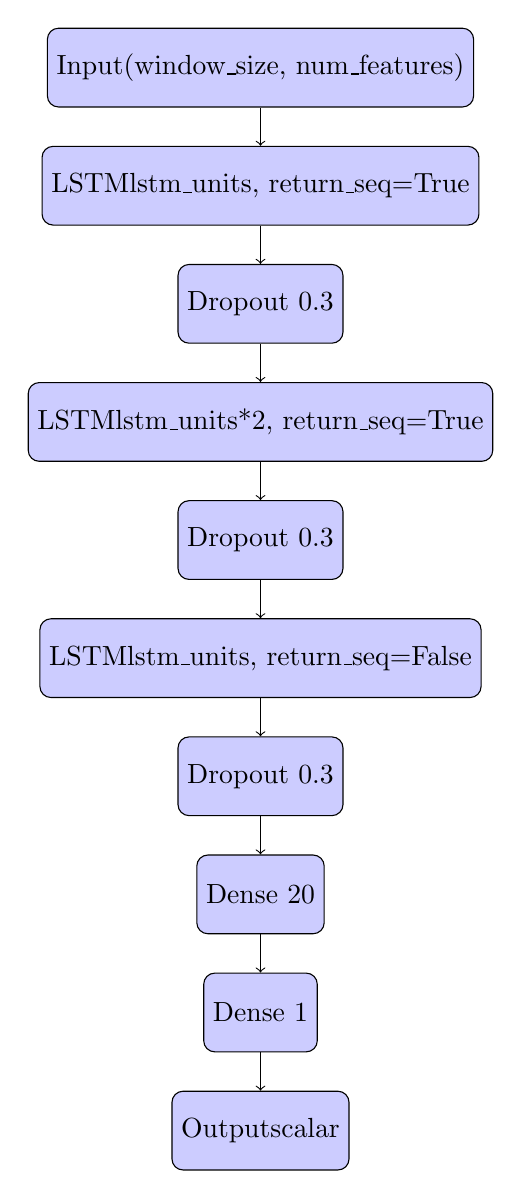
\begin{tikzpicture}[node distance=1.5cm, auto, thin]

\tikzstyle{block} = [rectangle, draw, fill=blue!20, text centered, rounded corners, minimum height=1cm]

% Nodes
\node[block] (input) {Input \\ (window\_size, num\_features)};
\node[block, below of=input] (lstm1) {LSTM \\ lstm\_units, return\_seq=True};
\node[block, below of=lstm1] (drop1) {Dropout 0.3};
\node[block, below of=drop1] (lstm2) {LSTM \\ lstm\_units*2, return\_seq=True};
\node[block, below of=lstm2] (drop2) {Dropout 0.3};
\node[block, below of=drop2] (lstm3) {LSTM \\ lstm\_units, return\_seq=False};
\node[block, below of=lstm3] (drop3) {Dropout 0.3};
\node[block, below of=drop3] (dense1) {Dense 20};
\node[block, below of=dense1] (dense2) {Dense 1};
\node[block, below of=dense2] (output) {Output \\ scalar};

% Connections
\draw[->] (input) -- (lstm1);
\draw[->] (lstm1) -- (drop1);
\draw[->] (drop1) -- (lstm2);
\draw[->] (lstm2) -- (drop2);
\draw[->] (drop2) -- (lstm3);
\draw[->] (lstm3) -- (drop3);
\draw[->] (drop3) -- (dense1);
\draw[->] (dense1) -- (dense2);
\draw[->] (dense2) -- (output);

\end{tikzpicture}
\end{center}

The optimal input parameters for the model were determined using a random search across batch sizes of 8, 16 and 32, epochs of 50, 100, and 150, and lstm\_units of 50, 100, 150.  At the end of each model generation the loss is determined and the model parameters that produced the minimal loss was chosen.  Given the data and parameters mentioned in this paper the optimal parameters was determined to be;

batch\_size: 16
epochs: 100
lstm\_units: 150

The loss for this model was 0.0006700601079501212 and the RMSE was 6.83 for equities and 0.09 for bonds.

\begin{figure}
    \centering
    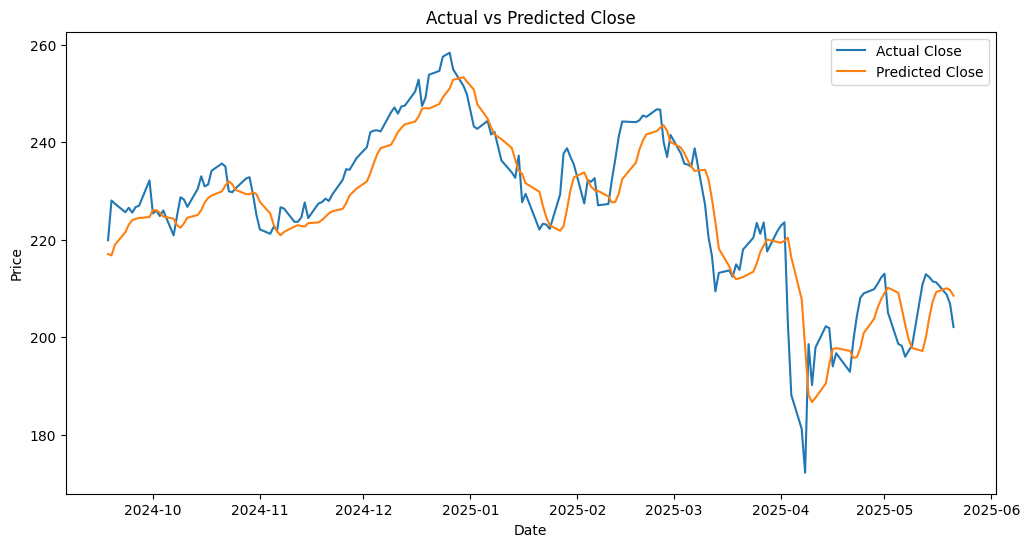
\includegraphics[width=1\linewidth]{lsmt_equity_actual_vs_predicted_close.png}

    \label{fig:enter-label}
\end{figure}

\section{Comparison}  

Our classical baseline model is \textbf{Ordinary Least Squares (OLS)}. While we can't compare different algorithms directly within this setup, we can evaluate OLS's in-sample performance and its pros and cons relative to other forecasting methods.  OLS offers clarity, computational efficiency, and interpretability through its summary and coefficients. It's an excellent linear baseline. However, its major limitation in financial forecasting is the assumption of linearity. Financial markets exhibit complex non-linear dynamics, which OLS often fails to capture, resulting in low values and limited explanatory power.

In contrast, another team member explored a different approach for financial forecasting. Their methodology incorporated a richer set of technical indicators for feature engineering, including the Relative Strength Index (RSI) and Moving Average Convergence Divergence (MACD), alongside longer-term moving averages (e.g., 60-day averages) to capture broader trends. For missing data, they employed various "fillers" for imputation. Crucially, their model aimed for more granular predictions: forecasting the next day's open, high, low, and close prices for both stocks and bonds, rather than just returns or price changes. This required handling multiple output targets, potentially through separate models or a multi-output regression framework. Their validation strategy involved "patch tests," effectively evaluating the model's performance over specific 60-day windows, providing a different perspective on its robustness compared to our single, in-sample OLS evaluation. While their approach involves a more complex feature set and prediction targets, it also highlights the diverse strategies required to tackle the multi-faceted nature of financial market predictions, suggesting avenues for future integration of advanced features and validation methods with our OLS baseline.

Compared to advanced models like neural networks (LSTMs) or tree-based methods (Random Forests), OLS is less capable of modeling intricate patterns and feature interactions. These more sophisticated algorithms, common in existing research, can learn non-linear mappings and potentially achieve better predictive accuracy, especially for volatile financial data. While higher-performing, they come with reduced interpretability and increased complexity. Our OLS implementation confirms linear signals and provides a foundational understanding, but the inherent difficulties with noisy financial data underscore the necessity of exploring non-linear modeling techniques in future work.

For the \textbf{PatchTST} model, we leveraged time-series patching for more effective temporal representation learning. This model used a sliding window of 90 days to forecast the next 30 days of closing prices. Compared to the simplicity of OLS, this model included OHCLV data and different technical indicators (MA5, MA20, RSI), to improve training stability. The PatchTST model performed multi-step forecasting which allowed it to learn long-term dependencies over time. When OLS was compared with PatchTST and LSTM, it was able to capture richer temporal dynamics due to its architecture and capacity, including when there were noisy and volatile market data. This model highlights the potential of neural networks in financial time series forecasting. 

\textbf{LSTMs} typically outperform simple linear regressions (OLS) on non-linear financial data. By learning gating mechanisms, they capture volatility clustering and regime-dependent effects that OLS misses. In empirical tests, LSTMs have beaten ARIMA/SVR baselines on stock returns[5] and have validated their memory advantage in bond yield tasks[6]. In a broad survey of deep learning in finance, LSTMs are often reported to excel (especially in hybrid setups with exogenous features)[7]. However, their accuracy gain depends on data volume and feature selection – an LSTM without useful inputs can under perform a well-tuned simpler model[8].

LSTMs are \textbf{not inherently interpretable}. The stateful weights and non-linear activations make it hard to trace how inputs map to outputs. LSTMs are often considered black boxes. Some recent work has “peeled” the LSTM by examining hidden-state activations: for example, Nunes et al. developed “LSTM-LagLasso” to link hidden-cell signals to economic variables, revealing some structure (e.g. certain units specialize for particular yield regimes)[9]. But these are post-hoc analyses. In general, an LSTM’s learned parameters offer no simple financial insight (unlike OLS coefficients)

LSTMs suit sequential data and can incorporate multiple inputs (prices, volumes, indicators). They can process daily equity or bond price sequences of varied length. Their gate structure helps avoid short-term volatility “noise” overwhelming the signal, making them useful even with highly auto-correlated data. They have fewer hyperparameters than transformers and can train on moderately sized datasets (e.g. 10+ years of daily data). For bonds, which often evolve more smoothly, LSTMs can capture yield-curve dynamics without many features. For equities, LSTMs require careful tuning and may benefit from additional inputs (technical indicators, macro factors) to improve signal.

LSTMs can \textit{overfit} easily on noisy daily data, especially if the signal-to-noise ratio is low. They require large amounts of data and careful hyperparameter tuning. LSTMs may also struggle with very long-horizon forecasts: studies note they “excel in short and medium-term patterns” but lose precision over longer horizons in volatile markets[10]. In volatile or rapidly changing markets, the LSTM’s training on past data may not generalize. Moreover, like any deep model, LSTMs can exhibit unstable behavior if their input distributions shift (e.g. a market crash). Computation time is also substantial compared to linear models. Overall, while LSTMs often beat OLS in accuracy, they share the “black box” limitation of deep learning and can fail if underlying market regimes shift or if the training series are too short or noisy[11][12].

\section{Future Directions}

While the current research is promising for LSTM based deep learning models other frontier models should be compared with the LSTM approach for a full understanding of how it compares with other SOTA models[14].  In addition, in order to see how these models perform, better real-world testing leveraging backtesting approaches as well as being incorporated into paper-trading environments would provide additional information that can be used to evaluate which models perform best.

While leveraging multiple frameworks has allowed us to compare their strengths and weaknesses it does make it more challenging to provide a true comparison of equals.  The same is true for aligning on underlying data and not leveraging synthetic bond data for the OLS model.  Aligning on the underlying data and leveraging additional methods to determine the model performance such as incorporating tensorboard[15] will allow for greater insight into how well the models were actually trained and allow for a more for a more equal comparison.

\section{Conclusion}

This paper investigates the application of deep learning techniques for time-series price prediction in financial markets, focusing on daily OHLCV data. The study compares three models: Ordinary Least Squares (OLS), Patch Time Series Transformer (PatchTST), and a custom Long Short-Term Memory (LSTM) architecture. Financial forecasting presents challenges due to the chaotic, noisy, and nonlinear nature of market data. While OLS provides a baseline with simplicity and interpretability, it struggles with capturing complex temporal dynamics. PatchTST leverages transformer-based architectures for long-range dependency modeling but faces limitations in volatile financial data with structural breaks. The custom LSTM model, designed to adapt to nonlinear dependencies and temporal variability, consistently outperformed both OLS and PatchTST across multiple assets, demonstrating superior generalization and stability under volatile conditions. Rigorous preprocessing and feature engineering were employed to ensure high-quality data inputs, and evaluation metrics such as Mean Squared Error (MSE), Mean Absolute Error (MAE), and directional accuracy assessed model performance. The results highlight the promise of LSTM-based approaches for financial forecasting, while also acknowledging the need for further exploration of hybrid models and real-world testing environments. Future work will focus on enhancing interpretability and robustness through interdisciplinary methodologies and advanced validation techniques.

\bibliographystyle{IEEEtran}
\bibliography{refs}

[1][4] Giantsidi, Sofia and Claudia, Tarantola, Deep Learning for Financial Forecasting: A Review of Recent Advancements. Available at SSRN: \href{https://ssrn.com/abstract=5263710}{https://ssrn.com/abstract=5263710} or \href{https://dx.doi.org/10.2139/ssrn.5263710}{http://dx.doi.org/10.2139/ssrn.5263710}

[2][5] \href{https://arxiv.org/html/2501.17366v1\#:~:text=technical\%20indicators\%2C\%20we\%20evaluated\%20these,which\%20showcased\%20its\%20ability}{License: CC BY-NC-SA 4.0} arXiv:2501.17366v1 [cs.LG] 29 Jan 2025

[3][6] \textbf{\href{https://arxiv.org/abs/2005.02217}{arXiv:2005.02217} [q-fin.CP]}

[7] \href{https://papers.ssrn.com/sol3/papers.cfm?abstract_id=5263710\#:~:text=snapshot\%20of\%20the\%20current\%20state\%2C,analysis\%20play\%20a\%20crucial\%20role}{papers.ssrn.com}

[8] \href{https://arxiv.org/html/2501.17366v1\#:~:text=technical\%20indicators\%2C\%20we\%20evaluated\%20these,which\%20showcased\%20its\%20ability}{arxiv.org}

[9] \href{https://arxiv.org/abs/2005.02217\#:~:text=what\%20we\%20develop\%20the\%20LSTM,require\%20smaller\%20input\%20sequences\%20and}{arxiv.org}

[10] \href{https://medium.com/@iamshahzu/understanding-lstm-networks-and-financial-forecasting-decoding-market-trends-with-deep-learning-6eb78a981be8\#:~:text=When\%20applied\%20to\%20financial\%20forecasting\%2C,term\%20forecasts.\%20Factors\%20such\%20as}{medium.com}

[11] \href{https://medium.com/@iamshahzu/understanding-lstm-networks-and-financial-forecasting-decoding-market-trends-with-deep-learning-6eb78a981be8\#:~:text=When\%20applied\%20to\%20financial\%20forecasting\%2C,term\%20forecasts.\%20Factors\%20such\%20as}{medium.com}

[12] \href{https://www.mdpi.com/2673-9909/5/3/76\#:~:text=models\%20demonstrate\%20promising\%20results\%20in,The\%20rapid\%20introduction\%20of\%20new}{mdpi.com}

[13] \href{https://www.mdpi.com/2673-9909/5/3/76\#:~:text=In\%20conclusion\%2C\%20stock\%20market\%20prediction,actionable\%20insights\%20in\%20this\%20domain}{mdpi.com}\href{https://www.researchgate.net/publication/380421292_Robustness_and_Interpretability_of_Machine_Learning_Models_in_Financial_Forecasting\#:~:text=The\%20field\%20of\%20financial\%20forecasting,innovations\%20because\%20of\%20the\%20ongoing}{researchgate.net}

[14] https://link.springer.com/chapter/10.1007/978-981-16-6893-7\_35

[15] https://www.tensorflow.org/tensorboard
\end{document}


